\documentclass[12pt,oneside,a4paper]{article}

\title{\textbf{Solar Tracker}}
\author{Enrico Sgarbanti - VR446095}

\usepackage{graphicx}
\usepackage{wrapfig}
% \usepackage{url}
\usepackage{hyperref}
\usepackage[italian]{babel}
\usepackage[utf8]{inputenc}

\begin{document}
\maketitle



\begin{abstract}
    Questo documento mostra la realizzazione di un semplice inseguitore solare ad un asse a scopo didattico realizzato con semplici componenti e un Arduino Nano.
\end{abstract}



\section{Introduzione}
L'obiettivo è riuscire a realizzare un dispositivo che sia in grado di ruotare rispetto ad un asse in modo da mostrare sempre la stessa faccia nel punto con più luce.



\section{Background}
Per la creazione di questo dispositivo sono state utilizzate varie competenze:


\subsection{Fotoresistenze}Le fotoresistenze hanno una resistenza inversamente proporzionale alla luce quindi maggiore è la luce e maggiore sarà il voltaggio letto (grazie alla legge di ohm V=RI).


\subsection{Partitore di tensione}
\begin{figure}[ht!]
    \centering
    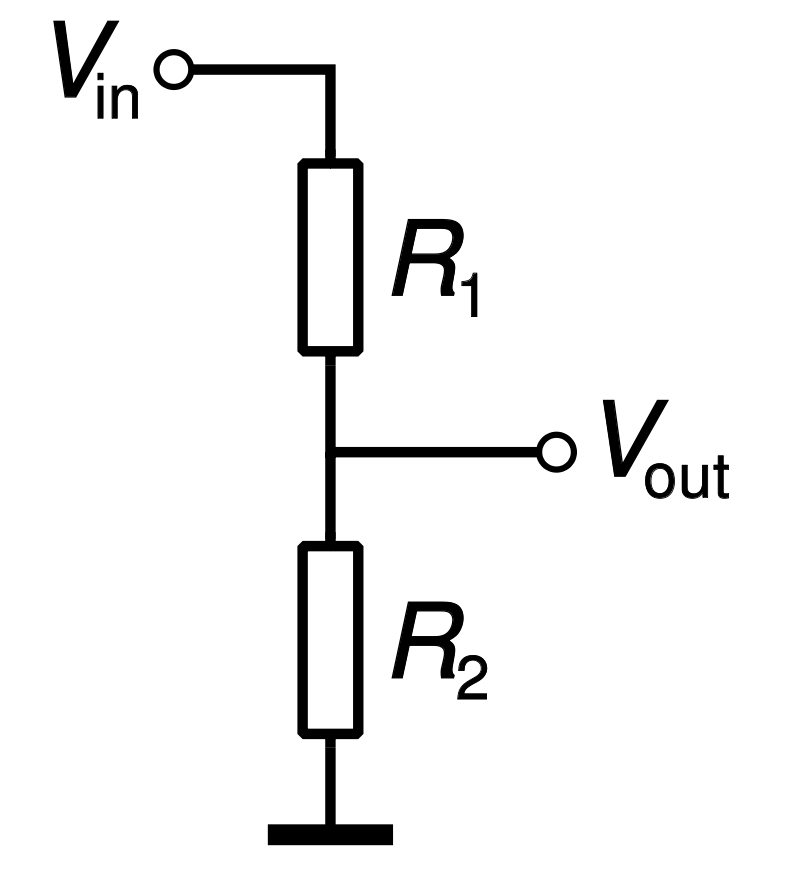
\includegraphics[width=0.3\textwidth]{figures/partitore_tensione.png}
    \caption{Partitore di tensione.}
\end{figure}
Il partitore di tensione\cite{VoltageDivider} è un tipo di circuito costituito da due o più componenti passivi collegati in serie ai capi dei quali, se viene applicata una tensione, essa si ripartirà sulle stesse componenti in base al loro valore.
Grazie all'applicazione della legge di Ohm e della legge di Kirchhoff si ricava che $V_{out} = V_{in} \frac{R_2}{R_1 + R_2}$.
\\Dalla formula si può notare che:
\begin{itemize}
    \item $V_{out} = \frac{V_{in}}{2}$ se $R_1 = R_2$.
    \item $V_{out} > \frac{V_{in}}{2}$ se $R_1 < R_2$.
    \item $V_{out} < \frac{V_{in}}{2}$ se $R_1 > R_2$.
\end{itemize}


\subsection{Motore passo-passo 4-fasi unipolare}
\begin{figure}[ht!]
    \centering
    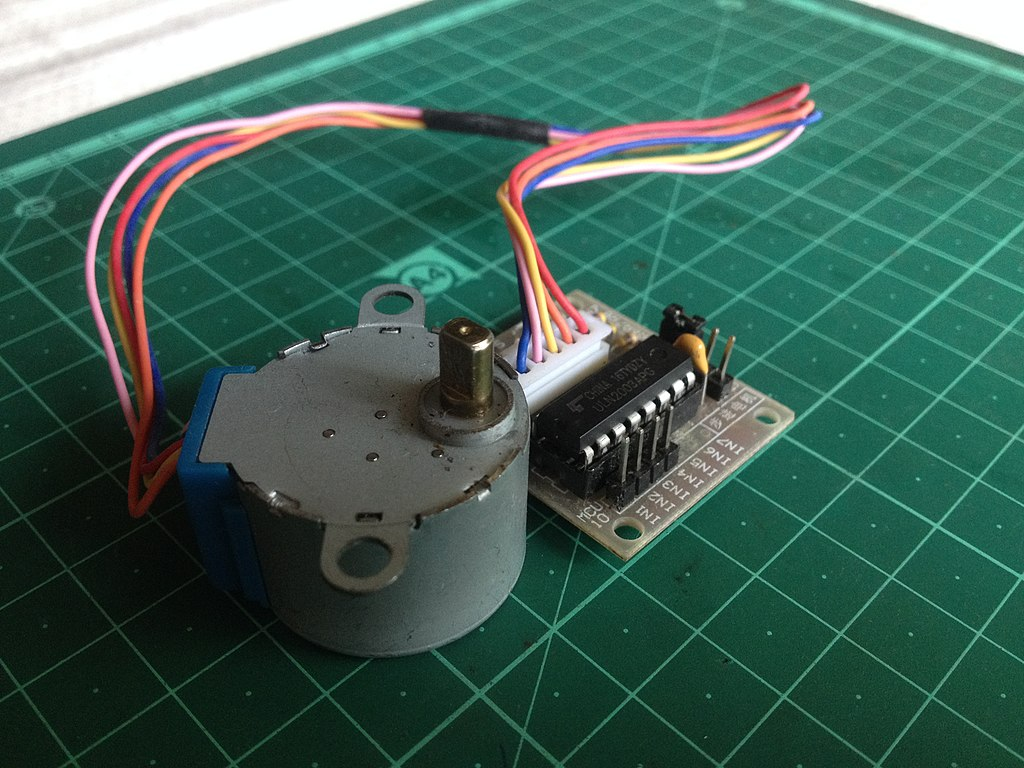
\includegraphics[width=0.5\textwidth]{figures/motor28BYJ-48.jpg}
    \caption{Motore 28BYJ-48.}
\end{figure}
Un motore passo-passo\cite{StepMotor} è un motore DC brushless che divide una rotazione completa in un numero di passi uguali.
A differenza degli altri motori, ha come scopo quello di mantenere fermo il rotore in una posizione di equilibrio: se alimentato si limita infatti a bloccarsi in una ben precisa posizione angolare. Per farlo muovere bisogna quindi inviare una serie di impulsi di corrente in un'opportuna sequenza. È così possibile far muovere il rotore nella posizione e alla velocità voluta semplicemente contando gli impulsi ed impostando la loro frequenza, visto che le posizioni di equilibrio del rotore sono determinate meccanicamente con estrema precisione.

\begin{figure}[ht!]
    \centering
    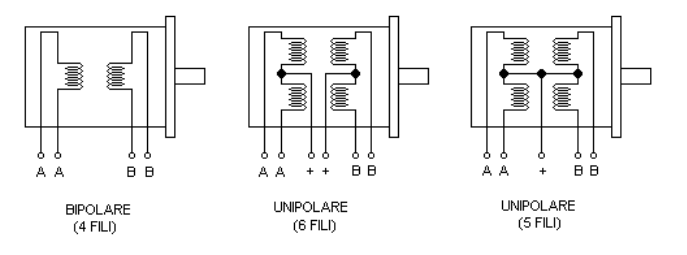
\includegraphics[width=0.5\textwidth]{figures/unipolare-bipolare.png}
    \caption{Struttura motori unipolari e bipolari.}
\end{figure}
I motori unipolari, rispetto a quelli bipolari, hanno uno o due fili in più che portano l'alimentazione e non necessitano di invertire la polarità sulle fasi.

\begin{figure}[ht!]
    \centering
    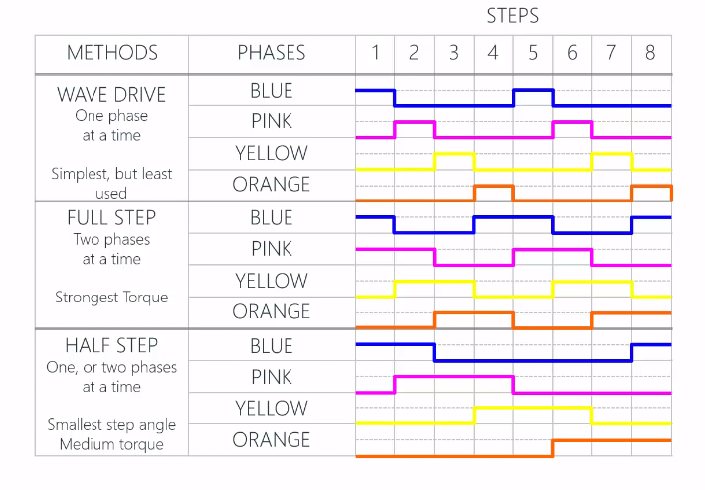
\includegraphics[width=0.5\textwidth]{figures/motor-sequence.png}
    \caption{Sequenza impulsi motore.}
\end{figure}
Un motore passo-passo è idealmente guidato da corrente sinusoidale. Sono state sviluppate varie tecniche di azionamento per approssimare meglio una forma d'onda di azionamento sinusoidale:
\begin{itemize}
    \item \textbf{Wave drive (una fase attivata): } Viene attiva una sola fase alla volta. Ha lo stesso numero di step dell'azionamento full-step, ma il motore avrà una coppia significativamente inferiore a quella nominale. È molto semplice, ma è usato raramente
    \item \textbf{Full-step drive (due fasi attive): } Vengono attivate due fasi alla volta. Sono sempre attive due fasi in modo che il motore fornisca la massima coppia nominale. Non appena viene disattivata una fase, ne viene attivata un'altra. Richiede più corrente, ma fornisce il doppio della coppia.
    \item \textbf{Half-stepping: } Si alterna tra una e due fasi. Viene attivata una fase, nel ciclo successivo un altra e in quello dopo viene disattivata la prima.  Richiede più corrente, ma fornisce una miglior precisione.
\end{itemize}


\subsection{Arduino}
\begin{figure}[ht!]
    \centering
    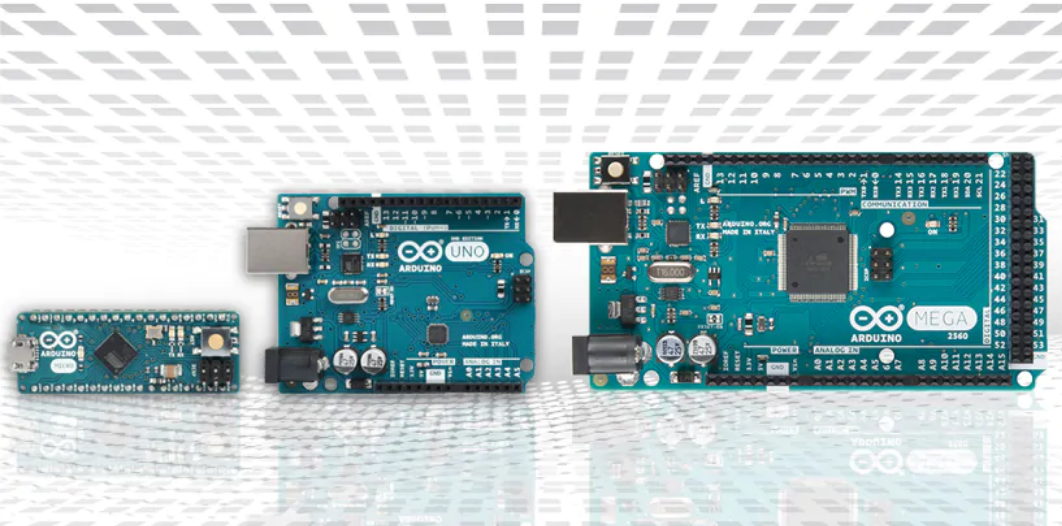
\includegraphics[width=0.5\textwidth]{figures/arduino.png}
    \caption{Schede Arduino Nano, Arduino UNO, Arduino Mega.}
\end{figure}
Arduino\cite{Arduino} è una piattaforma elettronica open source basata su hardware e software di facile utilizzo. Le schede Arduino permettono di leggere input da sensori, elaboratore i dati nel microcontrollore programmabile e restuire output mediante attuatori

\begin{figure}[ht!]
    \centering
    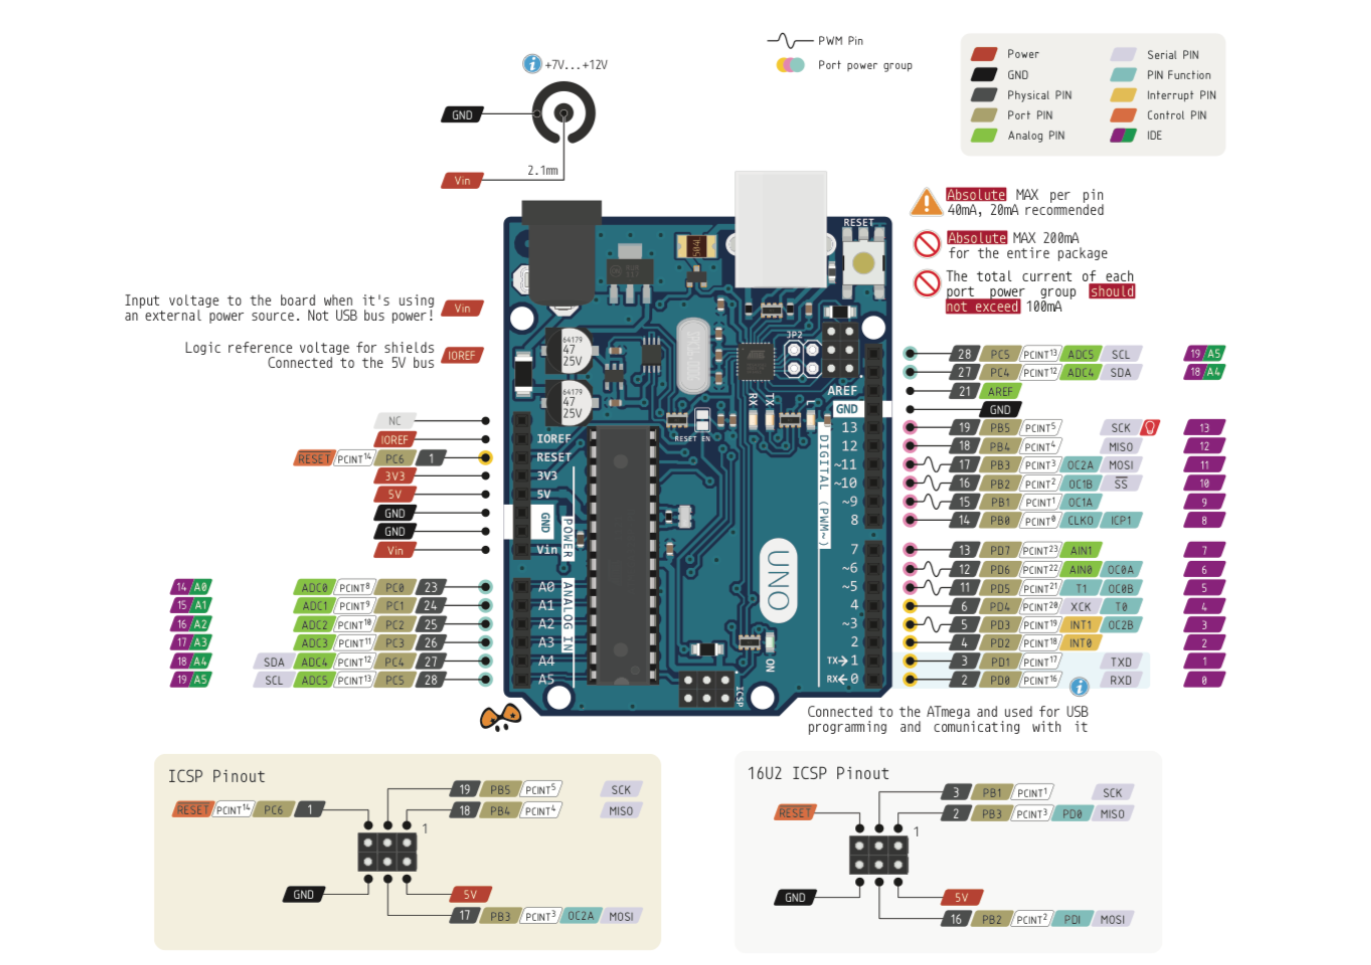
\includegraphics[width=0.5\textwidth]{figures/arduinoUNO.png}
    \caption{Arduino UNO.}
\end{figure}

\begin{figure}[ht!]
    \centering
    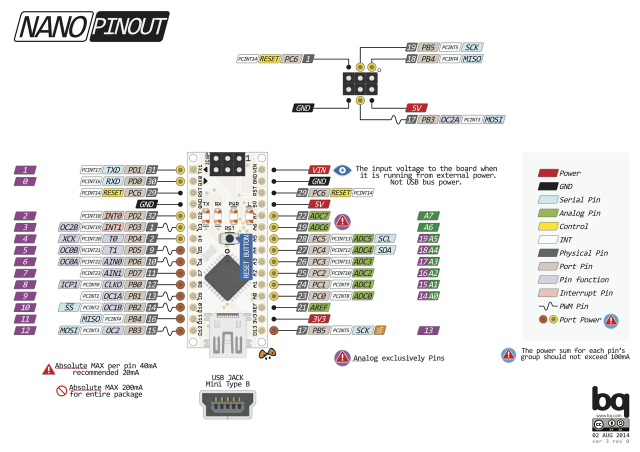
\includegraphics[width=0.5\textwidth]{figures/arduinoNANO.png}
    \caption{Arduino Nano.}
\end{figure}
Arduino è nato all'Ivrea Interaction Design Institute come uno strumento semplice per la prototipazione rapida, rivolto a studenti senza esperienza in elettronica e programmazione. Non appena ha raggiunto una comunità più ampia, la scheda Arduino ha iniziato a cambiare per adattarsi alle nuove esigenze e sfide, differenziando la sua offerta da semplici schede a 8 bit a prodotti per applicazioni IoT, indossabili, stampa 3D e ambienti incorporati. Tutte le schede Arduino sono completamente open-source, consentendo agli utenti di costruirle in modo indipendente e alla fine adattarle alle loro esigenze particolari. Anche il software è open source e sta crescendo grazie al contributo degli utenti di tutto il mondo.



\section{Solar Tracker}


\subsection{Struttura e componenti}
Il dispositivo è stato realizzato con:
\begin{itemize}
    \item 1x Arduino NANO
    \item 1x Stepper motor 28BYJ-48 \cite{MotorDatasheet}
    \item 1x Driver board ULN2003 \cite{DriverMotorDatasheet}
    \item 2x Photoresistor GL5537
\end{itemize}

\begin{figure}[ht!]
    \centering
    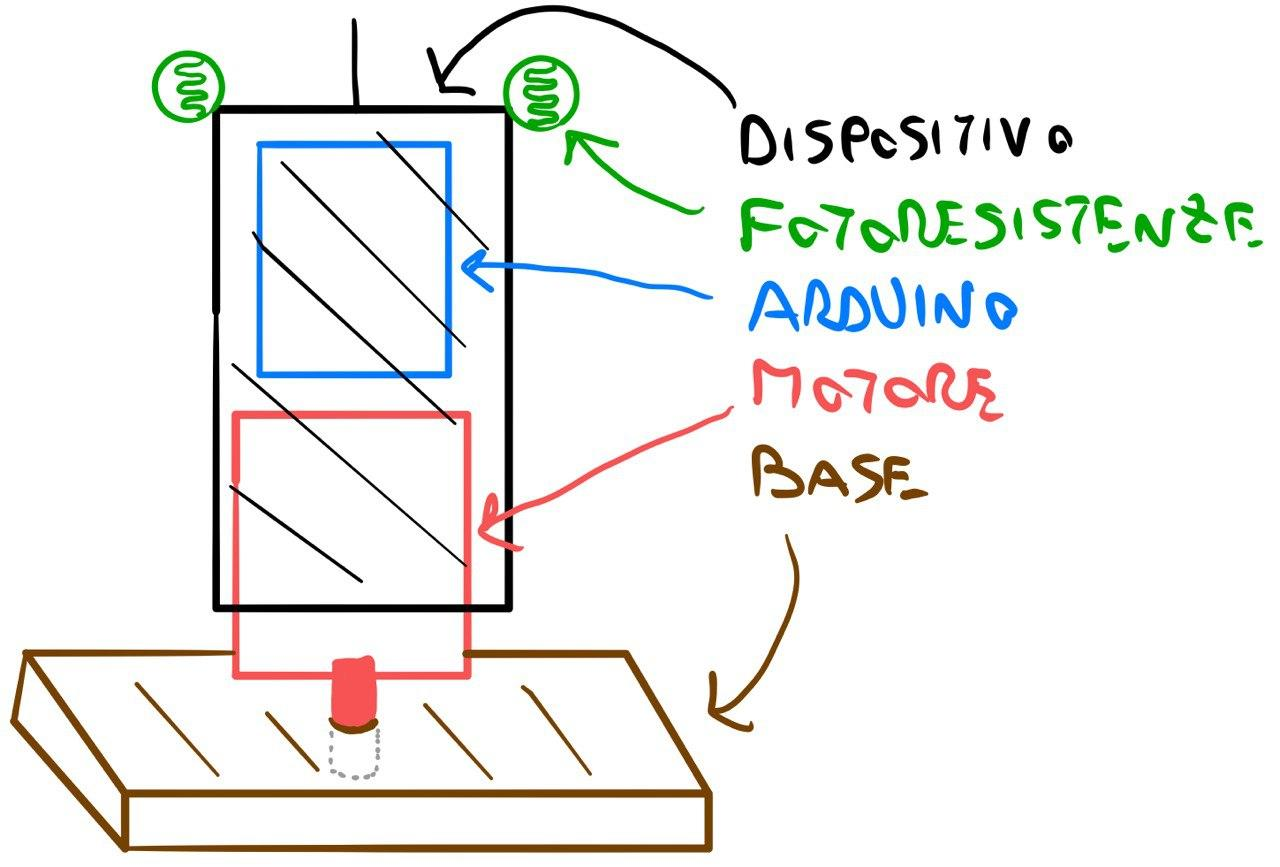
\includegraphics[width=0.5\textwidth]{figures/modello_solar_tracker}
    \caption{Struttura esemplificativa.}
\end{figure}
Al fine di permettere la completa rotazione, impossibile altrimenti a causa dei cavi, tutti i componenti sono stati disposti all'interno di una scatola tranne le fotoresistenze che si trovano nella parte superiore separate da un divisorio. (Il motore utilizzato non è il più adatto per questa scelta, ma essendo un prototipo a scopo didattico è stato utilizzato quello già visto a lezione)

\subsection{Funzionamento}
Ad un intervallo fissato l'Arduino inizierà a leggere il voltaggio generato dal partitore di tensione con le due fotoresistenze per muovere far muovere il motore fino a raggiungere la posizione di equilibrio ovvero quella in cui nella faccia del dispositivo è presente più luce.
L'intervallo fissato dipenderà dal tipo di applicazione, per esempio se lo scopo fosse quello di disporre un pannello solare sempre verso il sole allora sarebbe inutilmente dispendioso azionare l'Arduino ogni 10 secondi.

\subsubsection{Fotoresistenze}
\begin{wrapfigure}{R}{0.3\textwidth}
    \centering
    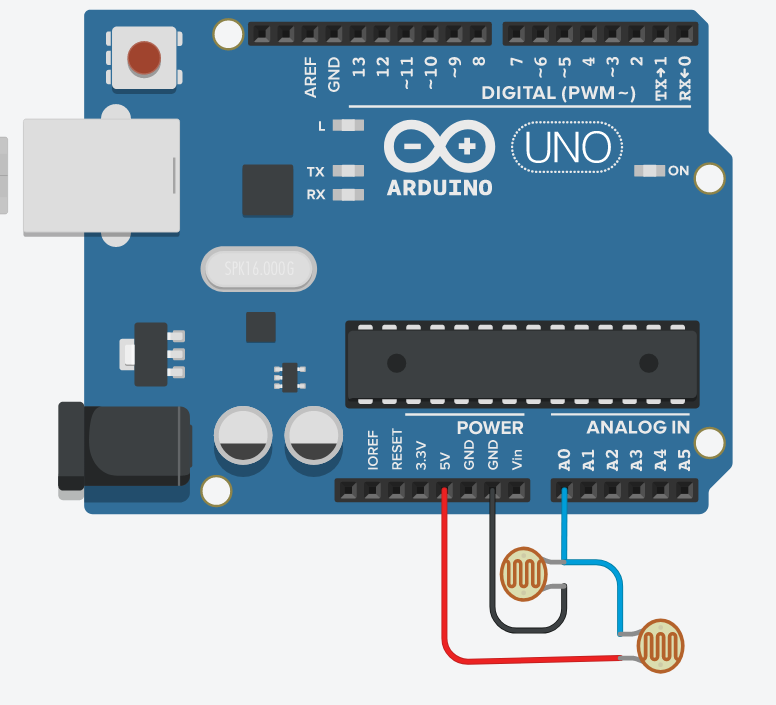
\includegraphics[width=0.25\textwidth]{figures/photoresistors}
    \caption{Collegamento fotoresistenze ad un Arduino UNO.}
\end{wrapfigure}
Grazie a due fotoresistenze dello stesso tipo è possibile trovare il punto in cui c'è più luce, ovvero quello in cui faranno la stessa resistenza.
Inserendole in un partitore di resistenza collegato ad un AnalogInput dell'Arduino diventa molto facile capire come spostarsi per trovare il punto di equilibrio, basterà leggere la tensione e:
\begin{itemize}
    \item se la tensione è 2.5V (cioè la metà dei 5V passati al partitore) allora le due fotoresistenze stanno facendo la stessa resistenza e quindi stanno ricevendo la stessa quantità di luce. Perciò si è arrivati alla posizione desiderata.
    \item se la tensione è maggiore di 2.5V allora la fotoresistenza collegata direttamente ai 5V sta facendo meno resistenza rispetto alla seconda e quindi è quella che sta ricevendo più luce.
    \item se la tensione è minore di 2.5V allora la prima resistenza sta facendo più resistenza rispetto alla seconda e quindi è quella che sta ricevendo meno luce.
\end{itemize}

\subsection{Elaborazione inputs}
Durante la ricerca del punto di equilibrio il dispositivo ad ogni ciclo deve leggere il valore di tensione data dalle fotoresistenze e dire al motore in che direzione andare fino alla lettura del valore di 2.5V. Essendo però difficile leggere esattamente il valore 2.500, il sistema risulterà instabile, continuando ad oscillare alla ricerca del punto di equilibrio. Per far fronte a questo problema, l'obiettivo non sarà più che l'input sia uguale a 2.5V ma minore di $2.5 - |epsilon|$ Volt.
Un primo approccio vede epsilon come numero fisso, ma questo valore dipende da vari fattori. Un secondo approccio che supera queste limitazioni vede epsilon come numero variabile, che partendo da 0 cresce ogni volta che c'è una inversione di rotazione.


\subsection{Utilizzo del motore}
Il motore utilizzato è un motore passo-passo unipolare a 4 fasi che è collegato ad una driver board che permette di controllarlo facilmente alimentando i quattro input.
\\La tecnica utilizzata per l'avanzamento è la full-step, in quanto la più consigliata.


\subsection{Considerazioni}
Aggiungendo un altro motore è possibile estendere la ricerca della posa con più luce tenendo conto di tutte e 3 le dimensioni.
Grazie a questo miglioramento è possibile realizzare un dispositivo che permetta ad un pannello solare di essere posizionato sempre nella posizione che dia la maggior efficienza.


\bibliographystyle{ieeetr}
\bibliography{biblio}


\end{document}